\chapter {Related Works}
\label{chap:related-works}

\section{Fully Supervised Semantic Segmentation}
\label{sec:fully-supervised}

In fully supervised semantic segmentation, the model is trained on a dataset with pixel-level annotations. The model learns to predict the class of each pixel in an image based on the provided annotations. This approach typically requires a large amount of labeled data, which can be expensive and time-consuming to obtain.

\subsection{Early Approaches}
\label{subsec:early-approaches}
The early approaches to semantic segmentation relied heavily on hand-crafted features and traditional machine learning techniques. These methods often involved extracting low-level features such as color, texture, and shape from the images and then using classifiers like Support Vector Machines (SVMs) or Random Forests to assign labels to each pixel.

Then came the era of deep learning, where convolutional neural networks (CNNs) revolutionized the field. The introduction of fully convolutional networks (FCNs) allowed for end-to-end training of segmentation models, enabling them to learn spatial hierarchies of features directly from the data. This was a significant breakthrough, as it eliminated the need for manual feature extraction and allowed for more accurate and efficient segmentation.

\subsection{Convolutional Neural Networks (CNNs)}
\label{subsec:cnn_sem_seg}

The first fully convolutional network (FCN) for semantic segmentation was proposed by \cite{fsss_fcn}, which replaced the fully connected layers in traditional CNNs with convolutional layers. This allowed the network to produce dense predictions for each pixel in the input image. The FCN architecture was further improved by adding skip connections, which helped to preserve spatial information and improve segmentation accuracy.

Then came the introduction of U-Net \cite{fsss_unet}, a popular architecture for semantic segmentation that is widely used in medical imaging and other applications. U-Net consists of an encoder-decoder structure, where the encoder captures context information and the decoder enables precise localization. The \emph{skip connections} between the encoder and decoder blocks play a crucial role by retaining spatial information, making U-Net particularly effective for tasks with limited training data.

The field of semantic segmentation has continued to evolve, with the introduction of various architectures and techniques.

The deeplab series \cite{fsss_deeplabv1, fsss_deeplabv2, fsss_deeplabv3,fsss_deeplabv3plus} introduced atrous convolution and spatial pyramid pooling to capture multi-scale context information; \cite{fsss_deeplabv1} also used a methd called CRF (Conditional Random Field) to refine the segmentation results. But it was removed in the later versions of the model. In \cite{fsss_deeplabv2}, the atrous convolution method evolved into a more general form called atrous spatial pyramid pooling (ASPP), which allows the model to capture features at multiple scales. The ASPP module consists of parallel atrous convolutions with different rates, enabling the model to learn multi-scale context information effectively. Finally \cite{fsss_deeplabv3plus} introduced a new decoder module that refines the segmentation results by combining low-level features from the encoder with high-level features from the ASPP module. This approach improves the localization of object boundaries and enhances the overall segmentation performance.

\cite{fsss_pspnet} introduced the Pyramid Scene Parsing Network (PSPNet), which uses a pyramid pooling module to capture global context information at different scales. The pyramid pooling module aggregates features from different regions of the image, allowing the model to learn rich contextual information for better segmentation.

\cite{fsss_segnet} proposed SegNet, an encoder-decoder architecture that focuses on efficient upsampling of feature maps. SegNet uses a series of convolutional and pooling layers in the encoder to extract features, followed by a corresponding decoder that upsamples the feature maps to produce the final segmentation output. The main innovation in SegNet is the use of unpooling layers, which store the indices of the max-pooling operation during encoding, instead of the feature maps themselves. This allows for more efficient memory usage and faster inference times, making SegNet suitable for real-time applications.

\subsection{Transformers}
\label{subsec:transformers}
The introduction of transformers in computer vision has led to significant advancements in semantic segmentation. Vision Transformer (ViT) \cite{transformer_vit} and its variants have shown promising results in various tasks, including semantic segmentation. ViTs leverage self-attention mechanisms to capture long-range dependencies and global context information, making them suitable for dense prediction tasks.
The years later on, the transformer-based architectures have gained popularity in semantic segmentation. \cite{transformer_swin} proposed the Swin Transformer, which introduces a hierarchical architecture with shifted windows to capture both local and global context information. The Swin Transformer has shown state-of-the-art performance on various benchmark datasets, including ImageNet-1k \cite{dataset_imagenet} for image classification and COCO \cite{dataset_coco} for object detection and \cite{dataset_ade20k} for semantic segmentation. The Swin Transformer has been widely adopted in various applications.

Leveraging the strengths of Vision Transformer, \cite{fsss_setr} first proposed the SETR (Semantic Segmentation Transformer) architecture, which replaces the traditional CNN backbone with a transformer encoder. The SETR architecture consists of a ViT encoder that processes the input image and generates a set of feature maps, followed by a decoder that upsamples the feature maps to produce the final segmentation output. The SETR model has shown competitive performance on various benchmark datasets, demonstrating the effectiveness of transformers in semantic segmentation tasks.

\cite{fsss_segmenter} proposed the Segmenter architecture, which combines a ViT backbone with a lightweight decoder for efficient semantic segmentation. The Segmenter model uses a transformer encoder to capture global context information and a simple decoder to produce the final segmentation output. The Segmenter architecture is designed to be computationally efficient while maintaining high accuracy, making it suitable for real-time applications.

\cite{fsss_segformer} introduced SegFormer, a transformer-based architecture that combines the strengths of both CNNs and transformers for semantic segmentation. SegFormer uses a hierarchical transformer encoder to capture multi-scale features and a lightweight decoder to produce the final segmentation output. The SegFormer model has shown state-of-the-art performance on various benchmark datasets, demonstrating the effectiveness of combining CNNs and transformers in semantic segmentation tasks.

The field of semantic segmentation has seen significant advancements with the introduction of various architectures and techniques. The combination of CNNs and transformers has led to improved performance and efficiency in semantic segmentation tasks. As the field continues to evolve, we can expect further innovations and breakthroughs in this area.

\subsection{Problem with Fully Supervised Semantic Segmentation}
\label{subsec:problem-with-fully-supervised}
Fully supervised semantic segmentation has achieved remarkable success, largely driven by powerful models and richly annotated datasets. However, this success comes at a significant cost: acquiring dense pixel-level annotations is both expensive and time-consuming. Each image must be meticulously labeled, often requiring expert knowledge and hours of manual effort. This high annotation burden severely limits the scalability of fully supervised methods, especially for large or specialized datasets. To overcome this bottleneck, the research community has increasingly turned toward weakly supervised semantic segmentation (WSSS) — an approach that seeks to train effective segmentation models with minimal supervision.





\section{Weakly Supervised Semantic Segmentation}
\label{sec:weakly-supervised}
Fully supervised semantic segmentation depends on pixel-level segmentation masks annotated by humans. However, generating such dense annotations is tedious, time-intensive, and costly. Furthermore, crowd-sourced annotators must undergo special training to handle the complexity of pixel-level labeling, which restricts the scale and diversity of available datasets. Consequently, most curated datasets are limited to a small set of object categories. In contrast, unlabeled or weakly annotated images can be collected in abundance, at much lower cost and in shorter time. This has motivated research into weakly supervised semantic segmentation (WSSS) to make semantic segmentation models more scalable.


\section{Types of WSSS}
\label{sec:types-weakly-supervised}
A wide range of weak supervision have been explored, including bounding boxes, scribbles, points, image-level labels,  eye tracks, free-form squiggles, or noisy web tags. Bounding boxes provide rough object boundaries, offering useful localization cues, though they still require annotators to draw accurate boxes.  Scribble-based supervision allows annotators to roughly mark object regions without outlining exact object boundaries. Point supervision, by contrast, typically uses a single annotated pixel per object, giving coarse location information. While less costly than pixel-accurate masks, these methods still involve some level of manual annotation, making large-scale labeling expensive.


\section{Image-level Label based weak supervision}
\label{sec:image-level-label}
Image-level annotation is one of the most economical and efficient settings for weakly supervised semantic segmentation. In this context, every training image has its image class labels belonging to the objects present in the image but the locations of the objects are unknown. So, the challenge is to accurately assign image-level labels to their corresponding pixels.
 
Initial approaches attempted to train segmentation models directly from image-level labels \cite{dcnn}, but performance was unsatisfactory. Later methods introduced discriminative localization techniques such as Class Activation Maps (CAMs) \cite{cam}, which highlight class-relevant regions. These coarse cues were then refined using auxiliary information such as superpixels \cite{imagelevelpixel}, segmentation proposals \cite{imagelevelpixel}, or motion information from videos \cite{wsss_motion_cues}. Some works, such as Adversarial Erasing \cite{adversarial_erasing}, expanded object coverage progressively by iteratively searching new regions. Others, like Kolesnikov and Lampert \cite{kolesnikov2016}, trained networks to approximate the dense CRF \cite{krähenbühl} applied on CAMs for refinement.

Some approaches learn to predict affinity matrices at the pixel level [36], to refine the output of dCRF through random walk. AffinityNet \cite{wsss_affinitynet} predicts class-agnostic pixel affinities to propagate CAM activations via random walks. Similarly, Seeded Region Growing (SRG) \cite{srg} expands initial seed regions using similarity criteria, while its deep learning extension DSRG \cite{wsss_dsrg_deep_seeded_region_growing} leverages high-level semantic features to grow regions more effectively. P2P \cite{pixel_to_prototype} further narrows the supervision gap by using pixel-to-prototype contrastive learning. A common limitation, however, is that most of these CNN-based methods inherit the restricted locality of convolutional features.

Recent advances incorporate transformers into WSSS \cite{camtokens, getam}. TS-CAM \cite{camtokens} leverages the global information capturing ability of ViT by combining class-token attention with CAMs. \cite{getam} refines class-specific maps by using attention gradients. MCTformer \cite{wsss_MCTformer} expands this idea by embedding multiple class tokens to learn attention maps for different categories. AFA \cite{wsss_afa_affinity_from_attention} instead derives semantic affinities directly from attention maps to refine coarse pseudo-labels. FrozenCLIP \cite{wsss_frozen_clip} pushes this further by exploiting the frozen CLIP backbone to generate high-quality pseudo-labels, which are dynamically updated using a refinement module (RFM).


\section{Stages}
\label{sec:stages}

Weakly supervised semantic segmentation has two main solutions based on their training processes: multi-stage approaches \cite{instance_wsss,wsss_L2G,wsss_rib} and single-stage approaches \cite{wsss_reliability_does_matter, wsss_afa_affinity_from_attention}. 

\subsection{Multi Stage}
\label{subsec:multi-stage}

Multi Stage WSSS has multiple steps. Typically, a classification model is first trained to generate the CAM,  which are then converted into initial pixel-level pseudo labels. These pseudo labels are refined through affinity matrix and random walk propagation\cite{wsss_affinitynet, wsss_afa_affinity_from_attention}, or seeded region growing[SRG] or contrastive learning. Then these refined pseudo labels are used for supervising a segmentation model.

Du et al. \cite{pixel_to_prototype} introduced a pixel-to-prototype contrastive method that enforces semantic consistency at the feature level, leading to improved pseudo-label quality. MCTformer \cite{wsss_MCTformer} extended transformer-based models with multiple class tokens, enabling the generation of category-specific attention maps for refined CAMs. More recently, researchers have incorporated CLIP into the WSSS pipeline. For instance, CLIMS \cite{wsss_clims} used CLIP to highlight more complete object regions while suppressing confident background activations. Similarly, CLIP-ES \cite{wsss_clip_es} applied a softmax-based GradCAM \cite{cam_grad} guided by carefully designed text prompts, allowing CLIP to produce reliable pseudo labels for segmentation supervision.

\subsection{Single Stage}
\label{subsec:single-stage}

In single-stage weakly supervised semantic segmentation, the model tries to learn segmentation directly from weak supervision (like image-level labels) in one shot. A network is trained that produces segmentation outputs without going through separate phases of label generation and refinement. There’s no explicit intermediate step to improve pseudo labels — the model directly predicts segmentation maps during training based on weak supervision signals.

Earlier works in this line used ImageNet-pretrained backbones \cite{dataset_imagenet} to jointly optimize classification and segmentation, with most efforts devoted to improving supervision quality or constraining the learning process. AA\&AR \cite{wsss_aaar} proposed an adaptive affinity loss that facilitates semantic propagation within the segmentation branch. AFA \cite{wsss_afa_affinity_from_attention} introduced an affinity branch to refine CAMs online, yielding stronger pseudo labels during training. ToCo \cite{wsss_toco_token_contrast} further advanced this direction by employing token-level contrastive learning to mitigate over-smoothing in CAM generation, thereby providing better online supervision.

\section{Types of CAM}
\label{sec:types-of-cam}
CNNs are often regarded as “black-box” models due to the limited interpretability of their internal mechanisms. Zhou et al.\cite{cam} demonstrated that different CNN layers could function as unsupervised object detectors through Class Activation Mapping (CAM). Building on this, Grad-CAM\cite{cam_grad} combines the class-discriminative property of CAM with gradient-based visualization techniques to focus on fine-grained image details.

An extension of this method, Grad-CAM++~\cite{cam_gradpp}, improves both object localization and the handling of multiple object instances within the same image compared to prior approaches. It achieves this by assigning pixel-wise weights to the gradients of the output with respect to specific spatial locations in the final convolutional feature map. The method derives closed-form solutions for these weights, including exact higher-order derivatives for softmax and exponential activations. Importantly, Grad-CAM++~\cite{cam_gradpp} requires only a single backward pass, keeping computational cost comparable to earlier gradient-based methods while offering more informative visualizations.

LayerCAM~\cite{layer_cam} further advances interpretability by generating reliable activation maps not only from the final convolutional layer but also from shallower layers. This allows it to capture both coarse object localization and detailed fine-grained features, thereby offering a multi-scale perspective of object representation within CNNs.

Beyond CNN-based methods, attention-based interpretability has also been explored. \cite{attention_rollout}introduced attention rollout and attention flow to compute attention scores for input tokens at each layer. Both approaches recursively propagate attention from earlier layers, taking into account residual connections. Attention rollout assumes that token identities propagate linearly through attention weights, while attention flow models the process as a flow network and applies a maximum flow algorithm to compute maximum flow values and trace information flow from hidden embeddings to input tokens. Compared to raw attention maps, these methods provide token-level attention that shows stronger correlation with input-gradient-based importance scores.

RelevanceCAM~\cite{relevance_cam} introduces a new CAM variant that leverages Layer-wise Relevance Propagation (LRP) to compute weighting components. By doing so, it addresses the shattered gradient problem, which often leads to noisy saliency maps in intermediate layers. RelevanceCAM\cite{relevance_cam} demonstrates that not only the final convolutional layers but also intermediate and shallow layers, with smaller receptive fields, can capture class-specific features. This results in improved faithfulness and robustness of explanations, with superior localization of target objects in earlier layers compared to existing CAM-based techniques.

\section{Breakdown of the pipeline}
\label{sec:pipeline-breakdown}
\subsection{Backbone}
\label{subsec:backbone}

The architecture of AffinityNet \cite{wsss_affinitynet} relies on three DNNs: a classification network for generating CAMs, the AffinityNet module itself, and a segmentation network. All three share the same backbone. The backbone is a modified variant of Model A1 \cite{RevisitingResNET}, commonly referred to as ResNet38, which consists of 38 convolutional layers with wider channels. In this adaptation, the GAP and fully connected layers from the original design are removed, and the final three convolutional stages are replaced with atrous convolutions with stride 1. The dilation rates are adjusted so that the resulting feature maps maintain a stride of 8.

In DSRG \cite{wsss_dsrg_deep_seeded_region_growing}, the classification branch employs a slightly altered version of the 16-layer VGG model \cite{VGG16}, while the segmentation branch is built upon DeepLab-V2 \cite{fsss_deeplabv2}. Both are initialized with VGG-16 weights pre-trained on ImageNet.

AFA \cite{wsss_afa_affinity_from_attention} adopts the Mix Transformer (MiT) backbone introduced in SegFormer \cite{fsss_segformer}, which is more suitable for image segmentation tasks compared to the vanilla ViT. The MiT parameters are initialized using ImageNet-1k pre-trained weights.

ToCo \cite{wsss_toco_token_contrast} uses the ViT-Base (ViT-B) backbone initialized with ImageNet pre-trained weights. Within the ViT encoder, an auxiliary classification head is introduced to produce CAMs. These auxiliary CAMs are then used to form pseudo labels guiding the Pixel-Token Contrast (PTC) module, and also to generate proposals for cropping positive and negative local patches for the Cross-Token Contrast (CTC) module. The final CAM is generated through the classification layer and subsequently transformed into pseudo labels.

CLIP-ES \cite{wsss_clip_es} employs the CLIP ViT-B/16 backbone, where the image encoder extracts visual features and the text encoder extracts linguistic features. Since CLIP is pre-trained on roughly 400 million image-text pairs, it provides strong multimodal representations for segmentation.

The whole framework of FrozenCLIP \cite{wsss_frozen_clip} consists of four major components: a frozen CLIP backbone (comprising a ViT-Base/16 image encoder and a text encoder) \cite{transformer_vit}, a classification module for generating initial CAMs, a decoder for segmentation prediction, and a refinement module (RFM) to enhance CAMs into pseudo labels for supervision.

\subsection{CAM generation}
\label{subsec:cam-generation}
In AffinityNet \cite{wsss_affinitynet}, the CAM generation model has the following three layers added on the top of the backbone network: a 3x3 convolution layer with 512 channels to adapt to the target task, a global average pooling layer to aggregate feature maps, and a fully connected layer for classification. The class activation map is obtained by weighting the feature maps according to the corresponding class-specific weights in the FC layer.  These activation maps are normalized so that the maximum activation equals 1, and the background map is derived by subtracting the highest class activation of each pixel from 1.

In DSRG \cite{wsss_dsrg_deep_seeded_region_growing}, CAMs \cite{cam} are used to localize foreground objects.  In their classification network, the fully-connected classifier is applied to conv7 to generate a heatmap for each object class. Then the discriminative object regions, used as seed cues for the foreground, are obtained by applying a hard threshold to the heatmap. For localizing background seed cues, they selected the regions in normalized saliency maps whose pixels are with low saliency values as background.

AFA \cite{wsss_afa_affinity_from_attention} also relies on CAMs to provide initial pseudo labels. The maps are computed using the weighted contributions of feature maps from the classification layer, followed by a ReLU activation to suppress negative values. The outputs are scaled to the range [0,1], with an additional background score introduced to separate foreground from background.

In ToCo \cite{wsss_toco_token_contrast}, an auxiliary classification layer is added to extract semantic knowledge and generate CAMs. Here, patch tokens are first aggregated using global max pooling (GMP) and then passed through a fully connected layer, producing auxiliary CAMs that guide the learning process.

For FrozenCLIP \cite{wsss_frozen_clip}, image features are extracted using the frozen CLIP image encoder, while class-specific text prompts (foreground and background) are encoded via the CLIP text encoder. Both image and text encoders are frozen during training.  Then, the classification scores are generated by computing distances between pooled image features and text features. Based on classification scores, Grad CAM \cite{cam_grad} is utilized to generate the initial CAM.


\subsection{Pseudo Label Generation}
\label{subsec:pseudo-label-generation}
AffinityNet predicts convolutional feature maps in which the semantic affinity between two feature vectors is measured using their L1 distance. To train this network, semantic affinity labels are derived from CAMs. Specifically, confident foreground and background regions are identified, while ambiguous regions are treated as neutral. Pairwise affinities are then defined according to class labels — assigned as 1 for pixels of the same class, 0 for different classes, and ignored for neutral labels. Once trained, AffinityNet refines CAMs through a random walk guided by the semantic transition matrix, thereby enhancing CAM quality and producing more accurate pseudo segmentation labels.

In DSRG, pseudo labels are generated by expanding initial seed cues into unlabeled regions using the classical Seeded Region Growing (SRG) algorithm \cite{srg}. For each class, the seed cues are visited in row first manner and its 8-connectivity neighborhood pixels are checked for similarity criteria. If they satisfy the criteria , those pixels are added to the set of seed cues for that particular class, and this process is repeated for every object class. The dynamically updated seed sets act as supervision, continuously refining pseudo labels during training.

The AFA module computes semantic affinities directly by linearly combining multi-head attention outputs through an MLP layer. To ensure matrix symmetry, the affinity matrix is summed with its transpose, under the assumption that nodes with the same semantics should be equivalent. Supervision is provided by pseudo affinity labels derived from refined CAMs: pixels are assigned to the class with the highest activation, and affinities are set positive if two pixels share the same class, otherwise negative. These pseudo affinity labels supervise the affinity prediction process. The learned semantic affinities are then used in a random walk propagation to refine the CAMs.

In ToCo, auxiliary CAMs are segmented into pseudo token labels by applying two background thresholds, categorizing tokens into reliable foreground, background, and uncertain regions. Positive token pairs are defined as those sharing the same label, while others are treated as negative. To counteract over-smoothing, the Patch Token Contrast (PTC) module maximizes similarity between positive pairs of patch tokens and minimizes it for negative ones. Additionally, the Class Token Contrast (CTC) module enforces consistency across entire object regions by aligning representations of global and local class tokens. Specifically, it reduces the gap between projected global class tokens and projected local tokens cropped from uncertain or background regions, thereby improving pseudo label quality.

\subsection{Segmentation prediction}
\label{subsec:segmentation-prediction}
In AffinityNet, the segmentation model is constructed by adding two atrous convolution layers on top of the backbone. The segmentation predictions are then supervised using refined CAMs, which are generated by propagating pairwise pixel affinities.
For DSRG, once seed cues are obtained from initial CAMs, an image semantic segmentation network is trained with these cues. A balanced seeding loss is applied so that the network’s predictions are encouraged to match only the seed regions defined by the classification network, while ignoring unlabeled pixels. As training progresses, the seed cues are iteratively refined into pseudo labels, and the segmentation model is retrained with the updated supervision.
In ToCo, the segmentation decoder is deliberately simple, consisting of two 3×3 convolutional layers (each with dilation rate 5) followed by a 1×1 prediction layer. The pseudo labels produced by ToCo are passed through a Pixel-Adaptive Refinement (PAR) module, and the improved labels serve as supervision for the decoder to generate the final segmentation output.
For AFA, an MLP-based decoder head is employed. This head fuses features across multiple levels through lightweight MLP layers to produce segmentation predictions. The supervision is provided by refined pseudo labels obtained through affinity propagation.
In FrozenCLIP, segmentation is guided by a feature decoder that extracts intermediate outputs from each transformer block of the CLIP image encoder. For each feature map, a dedicated MLP is applied to generate enhanced feature representations, which are concatenated and then passed through a convolutional layer to form a fused feature map. This fused representation is subsequently processed by multiple stacked multi-head transformer blocks, producing the final segmentation prediction P.

\subsection{Refinement}
\label{subsec:refinement}
A major challenge in weakly supervised semantic segmentation is the generation of high-quality pseudo labels from weak annotations. The quality of these pseudo labels directly impacts the performance of the segmentation model. Therefore, refinement techniques are often employed to improve the quality of the pseudo labels. These techniques can include post-processing methods, such as conditional random fields (CRFs), or affinity based methods that leverage the relationships between pixels to refine the segmentation results.

AffinityNet \cite{wsss_affinitynet} is a notable example of a refinement technique that uses affinity information to improve the segmentation results. After generating initial CAMs from image-level labels, AffinityNet trains a CNN network to classify whether two adjacent pixels belong to the same semantic region. A random walk algorithm, using these affinities, then propagates object labels across the image, enhancing coherence of the segmentation masks.

AFA \cite{wsss_afa_affinity_from_attention} advanced this idea by showing that pixel affinities can be efficiently derived from attention maps of vision transformers, rather than training a separate affinity prediction network. Specifically, AFA extracts affinity information from the self-attention layers of the transformer backbone, using which it performs random walk propagation like AffinityNet. This approach simplifies the refinement pipeline and benefits from the strong semantic relationships already captured by attention mechanisms. In addition, it introduces the Pixel Adaptive Refinement (PAR) module, which uses local color and spatial information to further refine the initial pseudolabels. PAR is based on pixel adaptive convolution and less costly compared to DCRFs. It also dilates the kernels to cover a larger area, allowing it to capture more contextual information.

CLIP-ES \cite{wsss_clip_es} uses a similar approach, but instead of using the attention maps from the transformer, it uses the attention maps from the CLIP model. The CLIP model is a powerful vision-language model that has been shown to be effective in object detection and segmentation tasks. By leveraging the attention maps from the CLIP model, CLIP-ES is able to generate high-quality pseudo labels that are more accurate and robust than those generated by traditional methods. It uses the random walk propagation like AFA, along with a bounding box mask to mask certain affinities while covering more object regions.

Frozen CLIP \cite{wsss_frozen_clip} is another technique that uses the CLIP model to generate pseudo labels. In addition to using the attention maps from the CLIP model, it uses the decoder to generate pseudo labels. Since its backbone is frozen, it requires a decoder to enable the model to learn the affinities of the features. Then it weights the decoder affinities with the frozen CLIP attention maps to get the final affinity map. After that, it uses the random walk propagation with box mask like CLIP-ES and applies the PAR module of AFA to get the final segmentation pseudo labels.

\section{Some other background information}
\label{subsec:some-other-background-information}

\subsection{Multi-Modal Learning}
\label{subsec:multi_modal_learning}
Multi-modal learning involves integrating information from different modalities, such as images and text, to enhance model performance. By combining complementary cues from multiple sources, models can develop a deeper and more comprehensive understanding of the data. For instance, in classification tasks, leveraging both visual and textual data enables the model to capture more nuanced semantic relationships. A key advantage of this approach is the potential for zero-shot learning, where the model can recognize and classify images from previously unseen categories. This is accomplished by aligning visual features with corresponding textual descriptions, allowing the model to generalize beyond the training set. Such capabilities are particularly valuable, as classification often underpins many downstream applications.

\subsubsection{Contrastive Learning}
\label{subsec:contrastive_learning}
Contrastive learning is a self-supervised approach focused on learning representations by distinguishing between positive and negative pairs. The objective is to bring representations of related inputs (such as an image and its corresponding textual description) closer in a shared embedding space, while pushing apart representations of unrelated inputs. This is typically achieved using a contrastive loss function, which minimizes the distance between positive pairs and maximizes it for negative pairs. Such a strategy enables models to acquire robust, discriminative, and generalizable feature representations.

\subsubsection{Training Strategy}
\label{subsec:training_strategy}
The training strategy for multi-modal learning generally integrates both supervised and self-supervised techniques. Models are trained on large-scale datasets containing paired samples from different modalities, facilitating the learning of meaningful representations through methods such as contrastive learning. Data augmentation is commonly applied to enhance the diversity and robustness of the learned features, thereby improving the model's generalization to unseen data.

\subsubsection{Task-Agnostic Learning}
\label{subsec:task_agnostic_learning}
Task-agnostic learning refers to the development of representations that are not specialized for a single task but are applicable across a range of downstream applications. This is accomplished by focusing on learning generalizable features through training on diverse datasets and leveraging multi-modal information. As a result, models can adapt their learned representations to various tasks, including image classification, object detection, and image segmentation. This adaptability makes task-agnostic learning a valuable approach for constructing versatile and reusable models.

\subsection{Contrastive Language-Image Pre-Training (CLIP)}
\label{subsec:clip}

CLIP \cite{vl_clip} is a multi-modal learning framework that utilizes contrastive learning to align images and text within a shared embedding space. It is designed to acquire representations that generalize well across different tasks without the need for task-specific fine-tuning. By training on extensive datasets of image-text pairs, CLIP learns to capture meaningful associations between visual and textual modalities.

\subsection{CLIP Architecture}
\label{subsec:clip_architecture}

\subsubsection{CLIP Components}
CLIP comprises two principal components:

\begin{itemize}
    \item \textbf{Image Encoder}: Responsible for processing images and extracting feature representations. This typically involves a Swin Transformer, pooling layers, and additional modules to capture spatial hierarchies and relationships within image data.
    \item \textbf{Text Encoder}: Processes textual data and converts it into a format suitable for comparison with image features. It generally includes transformer layers and attention mechanisms to capture semantic relationships within the text.
\end{itemize}

CLIP is trained using a contrastive loss function that aligns image and text features in a shared embedding space. This enables the model to learn representations applicable to a variety of tasks, such as image classification, object detection, and image segmentation. In the context of this work, CLIP's capabilities are leveraged for weakly supervised semantic segmentation, which relies solely on image-level classification.

\subsection{Unified Contrastive Learning (UniCL)}
\label{subsec:unicl}

UniCL, or Unified Contrastive Learning \cite{vl_unicl}, is a multi-modal learning framework that extends the ideas of CLIP by unifying different contrastive learning strategies within a single architecture. This enables more effective and flexible learning from multiple modalities.

UniCL is more than a straightforward extension of CLIP; it introduces several important innovations to improve both performance and adaptability.

A key feature of UniCL is its unified approach to contrastive learning, integrating image-label and text-label associations into a joint image-label-text space. This unified framework allows the model to leverage more positive pairs during training. While CLIP treats only the provided image-text pair as a positive match, UniCL recognizes that multiple text descriptions or images can correspond to the same category. For instance, both "a photo of a cat" and "a photo of a kitten" may be valid positive pairs for an image of a cat. UniCL’s contrastive loss encourages the model to learn similarities across all features sharing the same category, resulting in a more comprehensive and robust shared representation space for images and text.

\subsubsection{Unified Image-Text-Label Contrast in UniCL}
\label{subsec:unified_image_text_label_contrast}

UniCL employs a bidirectional learning objective between image-text pairs:
\begin{equation} \label{eq:unified_image_text_label_contrast}
    \min_{\{\theta, \phi\}} \mathcal{L}_{\text{BiC}} = \mathcal{L}_{i2t} + \mathcal{L}_{t2i},
\end{equation}
where \(\mathcal{L}_{i2t}\) and \(\mathcal{L}_{t2i}\) are the image-to-text and text-to-image contrastive losses, respectively. And \(\theta\) and \(\phi\) are the parameters of the image and text encoders, respectively.

The image-to-text contrastive loss to align matched images in a batch with a given text is defined as:
\begin{equation} \label{eq:unicl_image_to_text_contrastive_loss}
    \mathcal{L}_{i2t} = - \sum_{i \in \mathcal{B}} \frac{1}{|\mathcal{P}(i)|} \sum_{k \in \mathcal{P}(i)} 
    \log \frac{\exp(\tau \mathbf{u}_i^\top \mathbf{v}_k)}{\sum_{j \in \mathcal{B}} \exp(\tau \mathbf{u}_i^\top \mathbf{v}_j)},
\end{equation}
where $k \in \mathcal{P}(i) = \{k | k \in \mathcal{B}, y_k = y_i\}$, i.e., the set of all images in the batch that belong to the same class as image $i$.

On the other hand, the text-to-image contrastive loss to align matched text in a batch with a given image is defined as:

\begin{equation} \label{eq:unicl_text_to_image_contrastive_loss}
    \mathcal{L}_{t2i} = - \sum_{j \in \mathcal{B}} \frac{1}{|\mathcal{P}(j)|} \sum_{k \in \mathcal{P}(j)} 
    \log \frac{\exp(\tau \mathbf{u}_k^\top \mathbf{v}_j)}{\sum_{i \in \mathcal{B}} \exp(\tau \mathbf{u}_i^\top \mathbf{v}_j)},
\end{equation}
where $k \in \mathcal{P}(j) = \{k \mid k \in \mathcal{B}, y_k = y_j\}$, i.e., the set of all text features in the batch that belong to the same class as text $j$.

\subsubsection{Comparison with CLIP}
\label{subsec:clip_vs_unicl}

In case CLIP, for an image, there is only one positive text feature. In other words, $\mathcal{P}(i) = {i} \in \mathcal{B}$; and $\mathcal{P}(j) = {j} \in \mathcal{B}$. So, the image-to-text contrastive loss is defined as:

\begin{equation} \label{eq:clip_image_to_text_contrastive_loss}
    \mathcal{L}_{i2t} = - \sum_{i \in \mathcal{B}} 
    \log \frac{\exp(\tau \mathbf{u}_i^\top \mathbf{v}_i)}{\sum_{j \in \mathcal{B}} \exp(\tau \mathbf{u}_i^\top \mathbf{v}_j)},
\end{equation}
where $i \in \mathcal{B}$ is the index of the image in the batch.

And the text-to-image contrastive loss is defined as:

\begin{equation} \label{eq:clip_text_to_image_contrastive_loss}
    \mathcal{L}_{t2i} = - \sum_{j \in \mathcal{B}} 
    \log \frac{\exp(\tau \mathbf{u}_j^\top \mathbf{v}_j)}{\sum_{i \in \mathcal{B}} \exp(\tau \mathbf{u}_i^\top \mathbf{v}_j)},
\end{equation}
where $j \in \mathcal{B}$ is the index of the text feature in the batch. 

The equations \ref{eq:unified_image_text_label_contrast}-\ref{eq:clip_text_to_image_contrastive_loss} are taken from \cite{vl_unicl}.

This means that $\mathcal{L}_{BiC}$ becomes CLIP training objective. The main property in \autoref{eq:unicl_text_to_image_contrastive_loss} is that for each image feature, any of the text features in the batch can be used as a positive pair. And so is the case for \autoref{eq:unicl_text_to_image_contrastive_loss}.

Second, UniCL replaces CLIP's ViT backbone with a Swin Transformer backbone. The Swin Transformer is a hierarchical vision transformer that captures both local and global information in images, making it more suitable for various vision tasks.

\subsection{Swin Transformer}
\label{subsec:swin_transformer}
Swin Transformer is a hierarchical vision transformer that employs a shifted windowing scheme to capture both local and global information in images. It is designed to be computationally efficient while maintaining high performance on various vision tasks. The architecture consists of multiple stages, each with its own set of transformer blocks, allowing it to process images at different resolutions and capture multi-scale features.

\autoref{fig:swin_vs_vit_architecture} illustrates the architectures of the Swin Transformer and Vision Transformers (ViT). The key distinction lies in their processing strategies: the Swin Transformer employs a hierarchical structure, processing feature maps at multiple resolutions, while ViT processes the entire image globally at a single resolution. This hierarchical approach enables the Swin Transformer to effectively capture both local and global information, making it particularly suitable for tasks requiring fine-grained details alongside overall context.

The Swin Transformer builds hierarchical feature maps by progressively merging image patches (depicted in gray) in deeper layers. It computes self-attention only within local windows (highlighted in red), resulting in linear computational complexity relative to the input image size. This efficiency, combined with its ability to handle dense recognition tasks, makes it a versatile backbone for both image classification and segmentation.

In contrast, traditional vision Transformers, such as ViT, produce feature maps at a single low resolution and compute self-attention globally, leading to quadratic computational complexity with respect to the input image size. This global attention mechanism, while effective for certain tasks, is less efficient for dense prediction tasks compared to the Swin Transformer's localized attention mechanism.

\begin{figure}[htbp]
    \centering
    \fbox{ % Draw a box around the entire figure
        \begin{minipage}{0.9\textwidth} % Adjust the width as needed
            \begin{subfigure}[b]{0.45\textwidth}
                \centering
                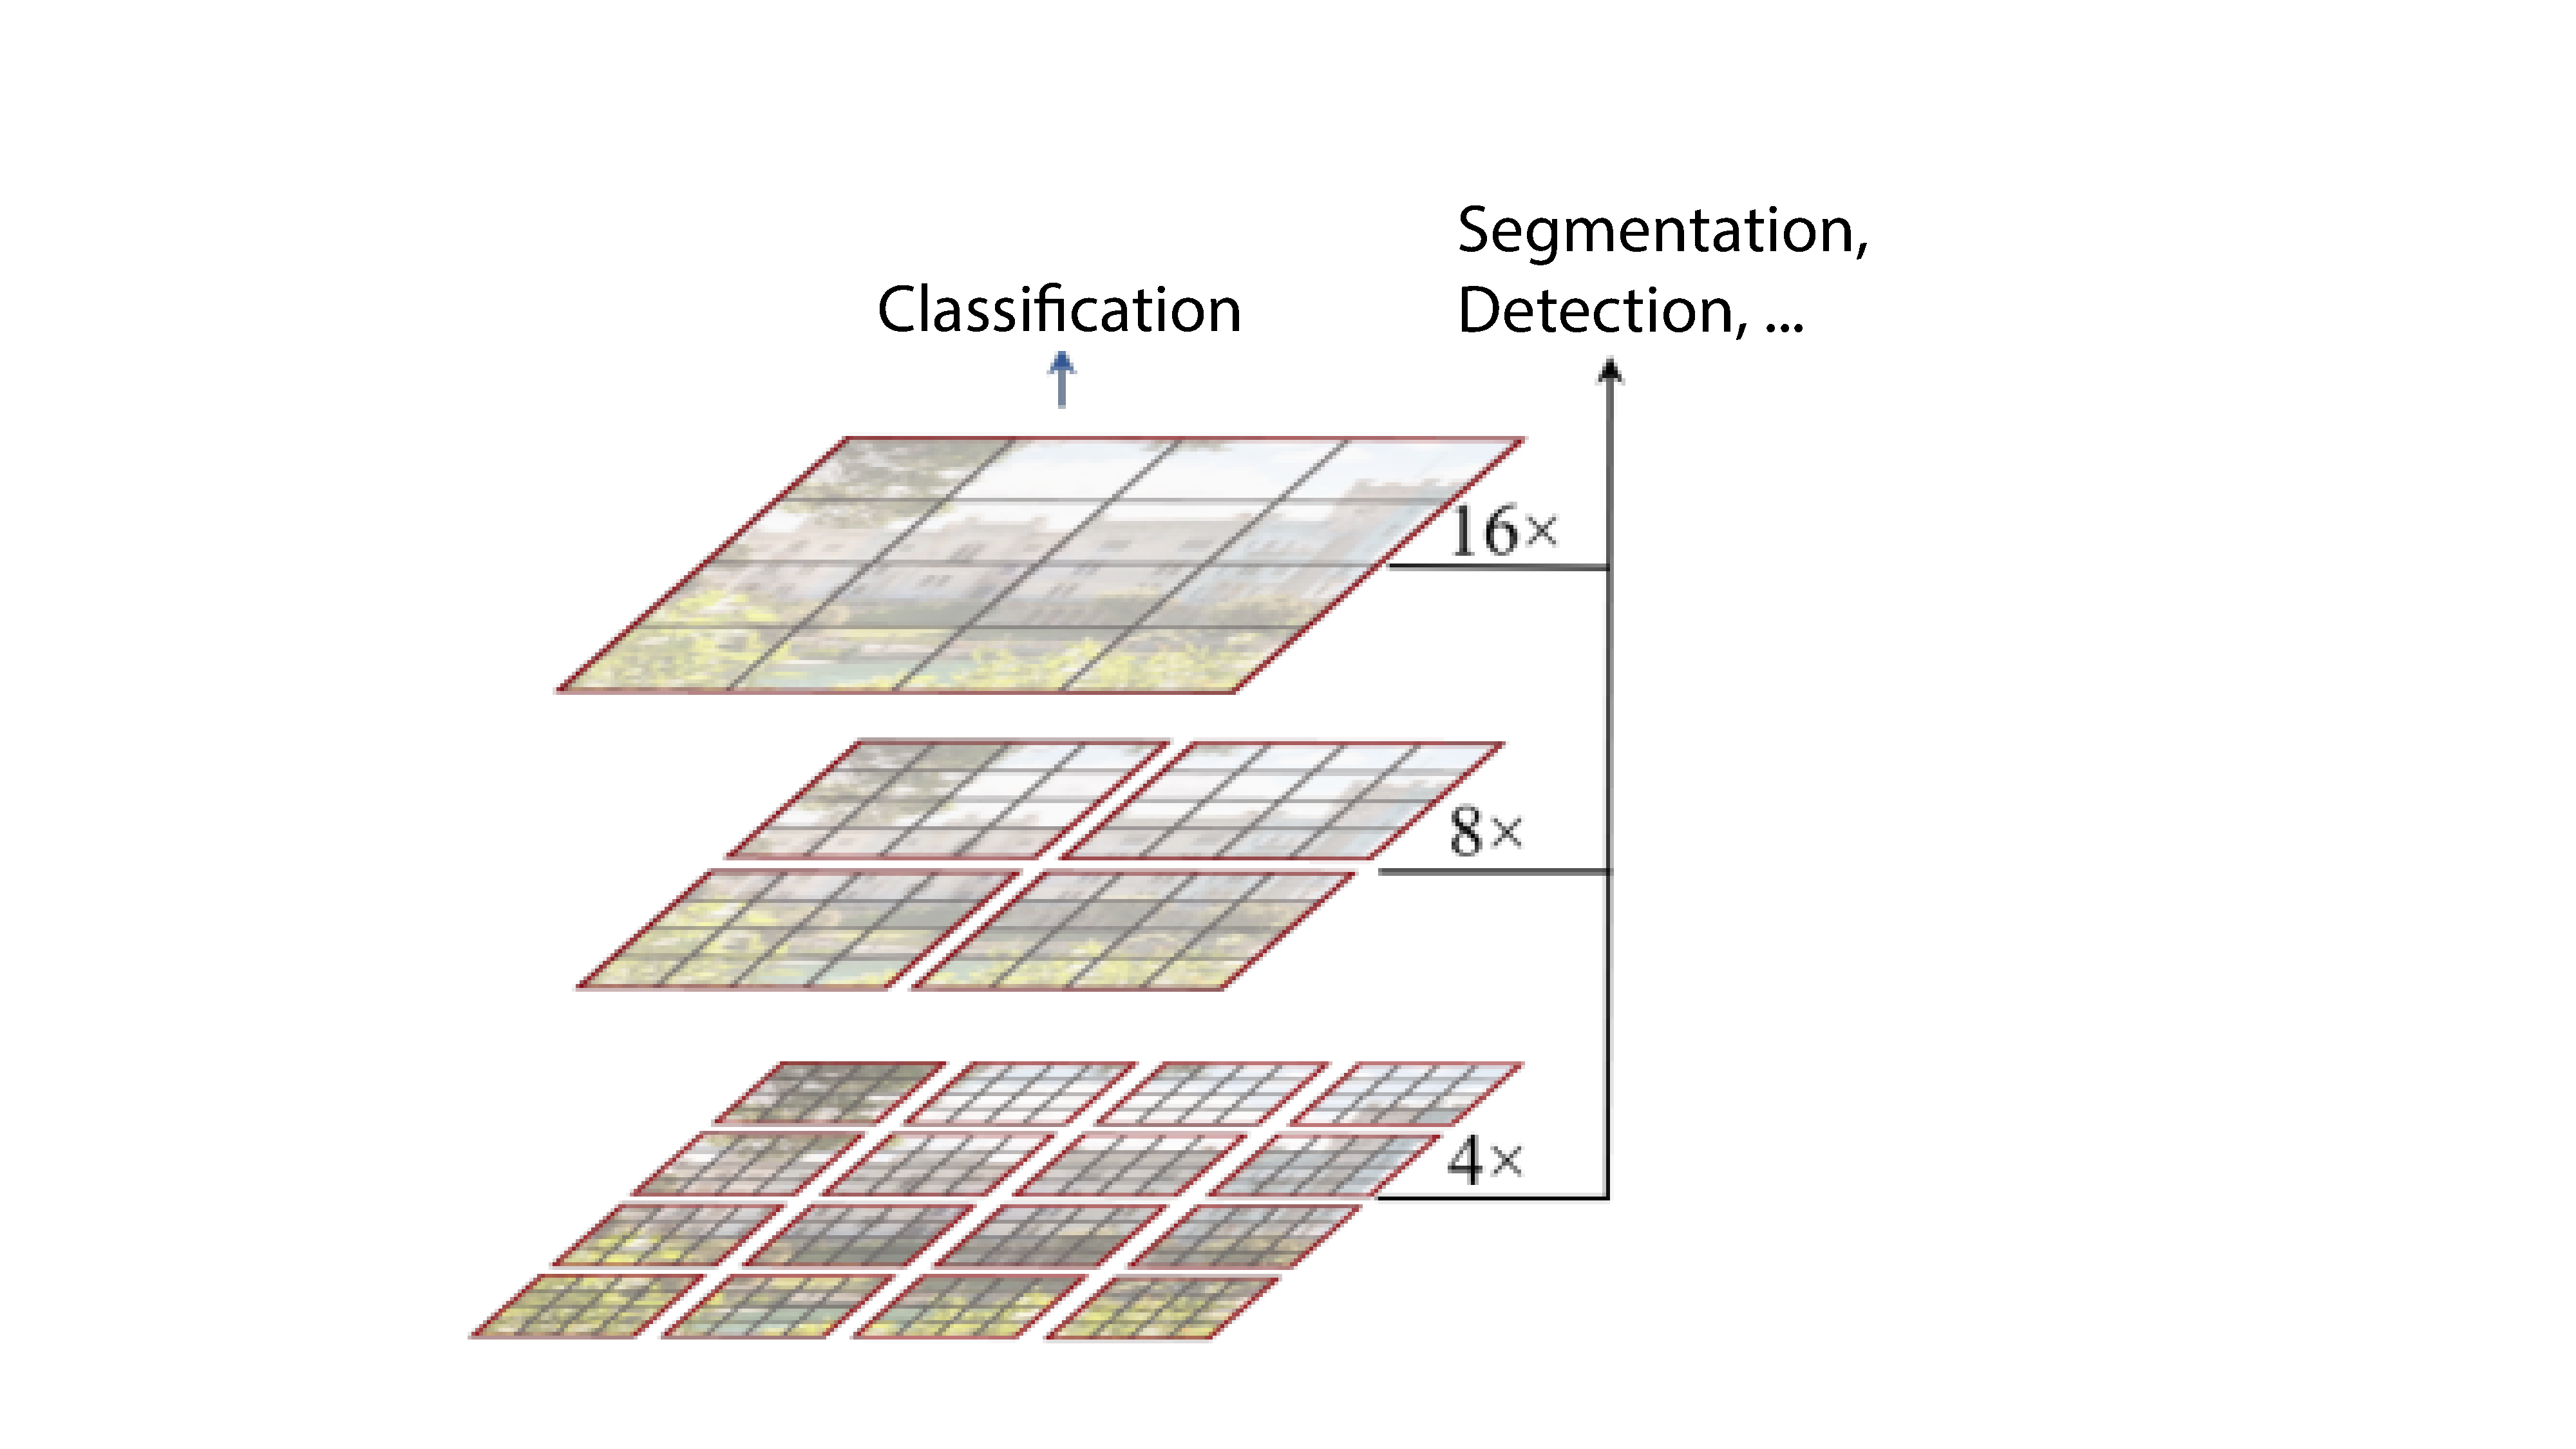
\includegraphics[width=\textwidth]{swin-vs-vit-archi-a.pdf}
                \caption{Swin Transformer}
                \label{fig:swin_transformer_data_flow}
            \end{subfigure}
            \hfill
            \begin{subfigure}[b]{0.45\textwidth}
                \centering
                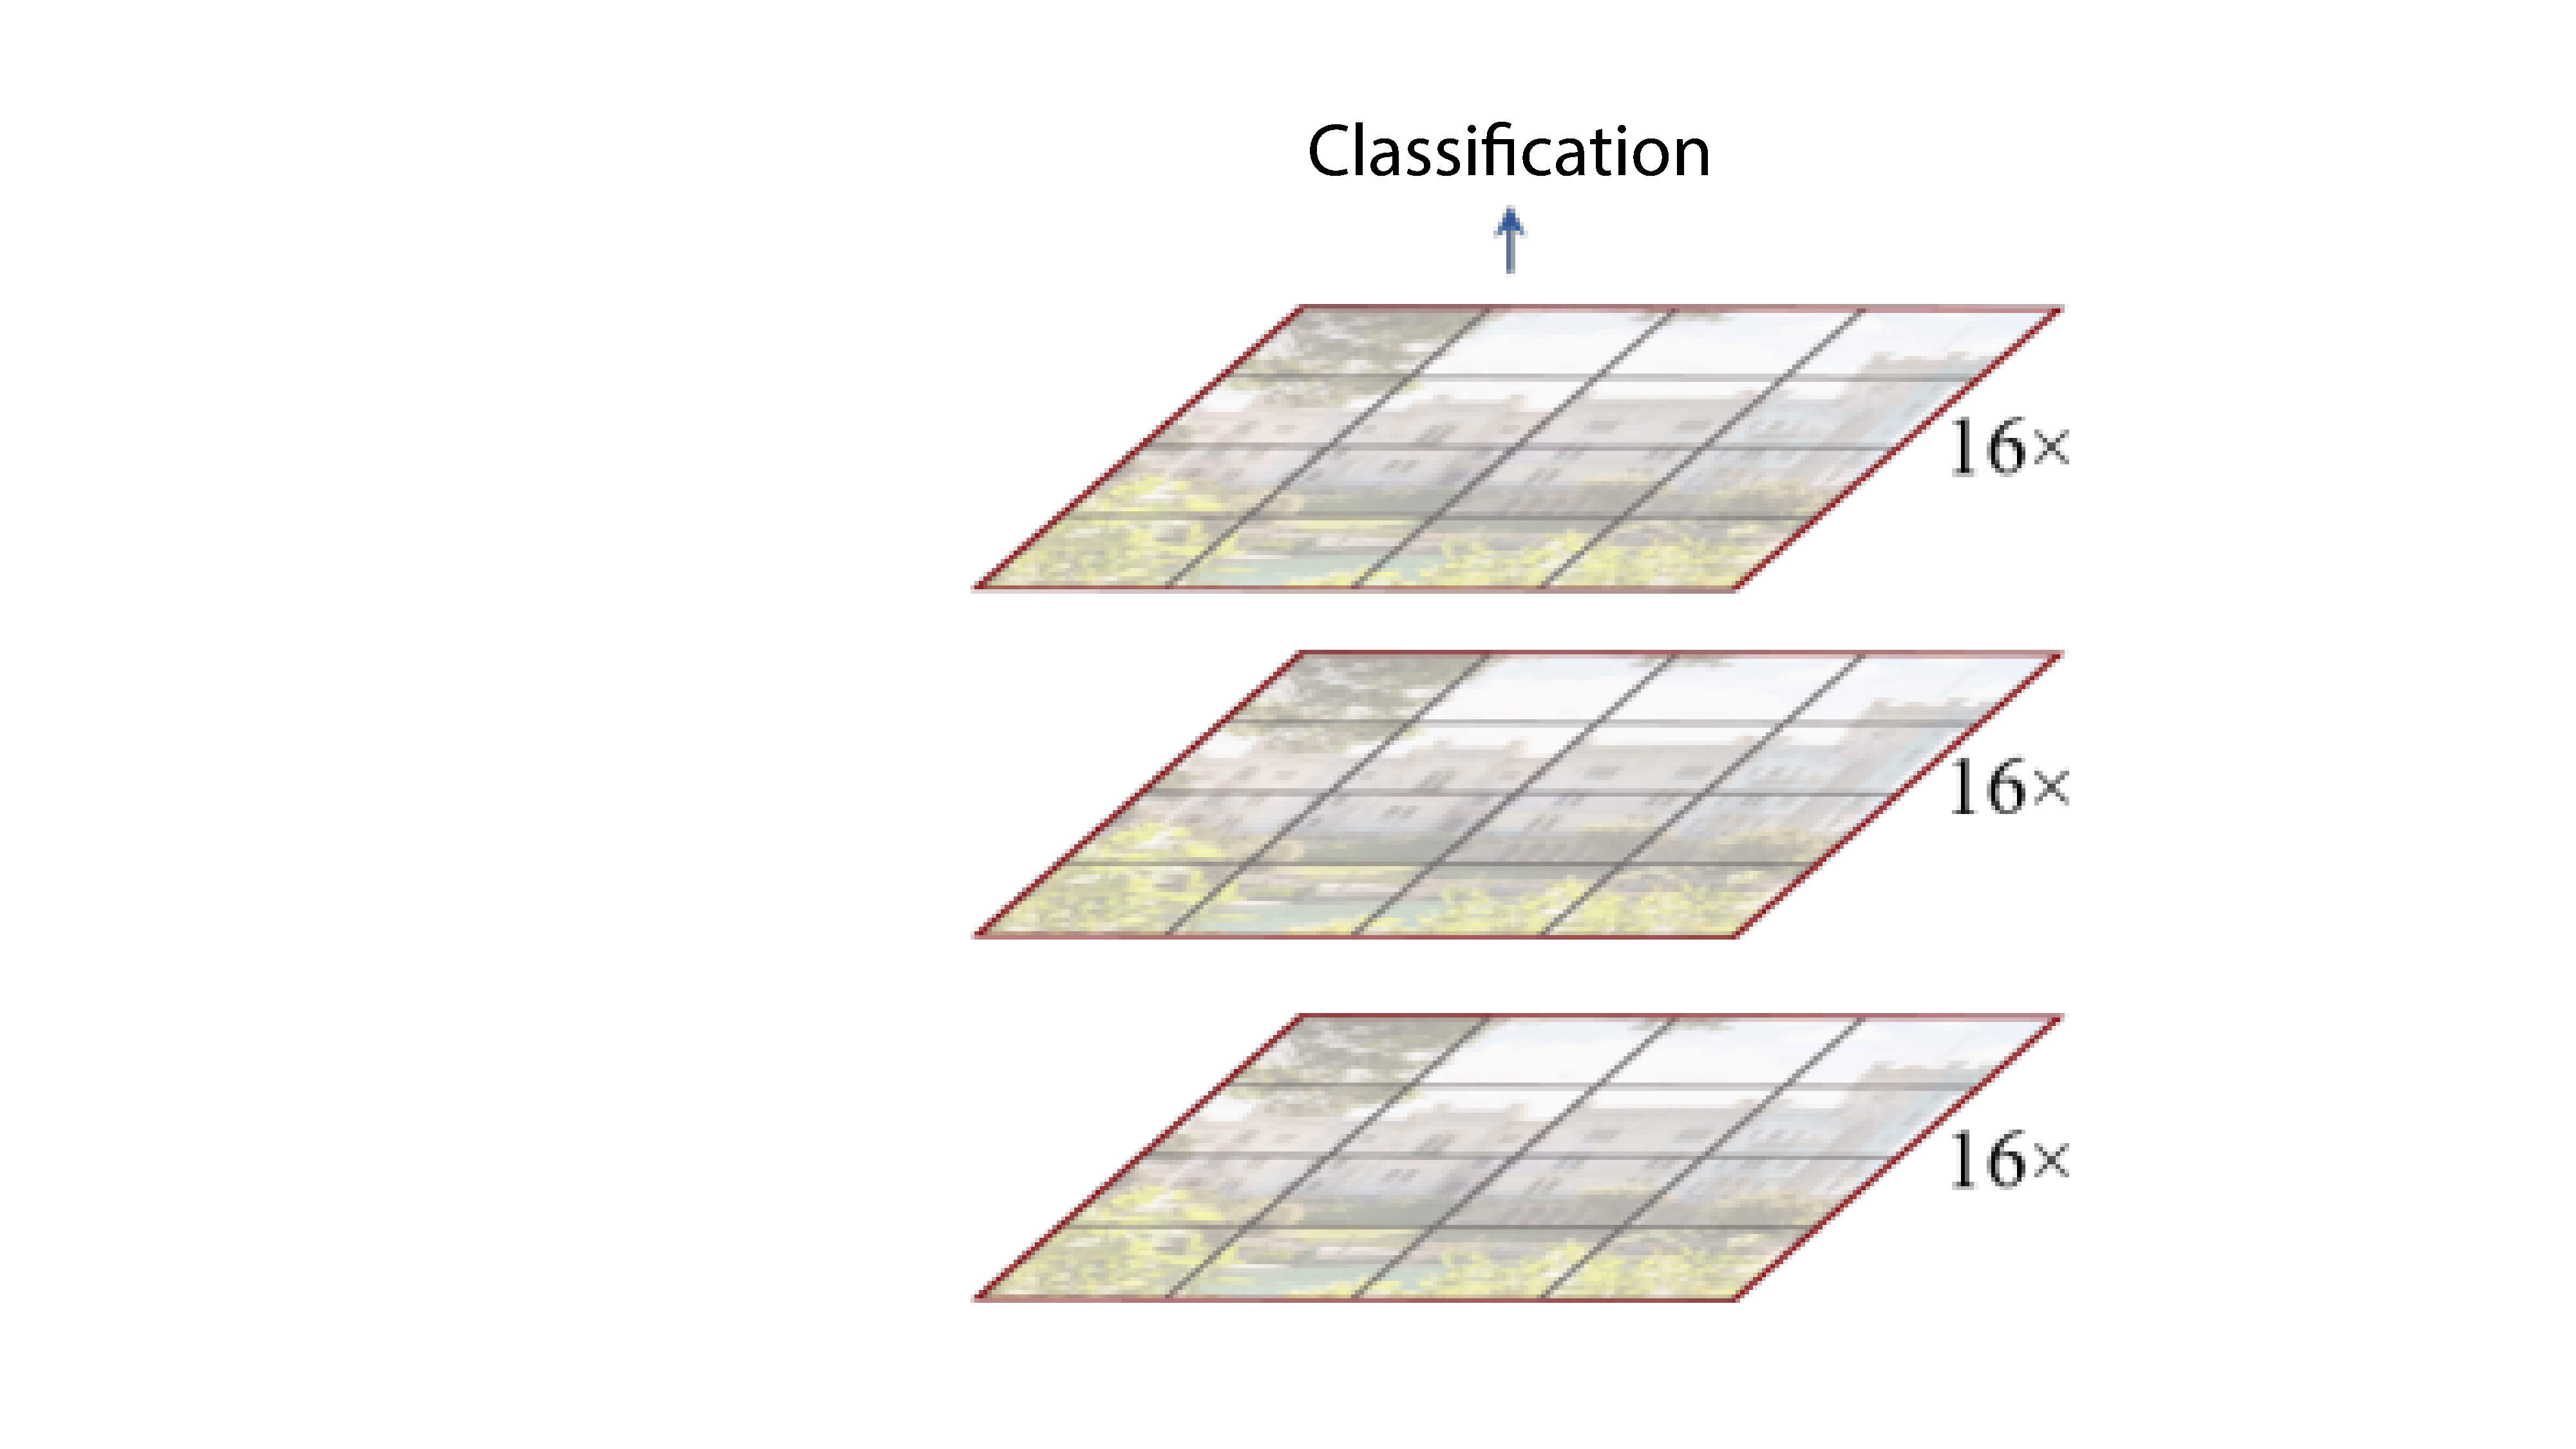
\includegraphics[width=\textwidth]{swin-vs-vit-archi-b.pdf}
                \caption{Vision Transformers}
                \label{fig:vit_data_flow}
            \end{subfigure}
        \end{minipage}
    }
    \caption{Comparison of Swin Transformer and ViT Architectures}
    \label{fig:swin_vs_vit_architecture}
\end{figure}

Because of the hierarchical nature of the Swin Transformer, it is particularly well-suited for tasks that require a combination of global context (to indentify the overall structure of the image) and local details (to capture fine-grained features, e.g., edges, textures). This makes it a strong candidate for image segmentation tasks.

Also, the Contrastive and Multi-Modal Learning capabilities of UniCL can be effectively combined with the Swin Transformer's hierarchical architecture to enhance the model's ability to learn rich and discriminative features from both image and text modalities. This combination allows for a more comprehensive understanding of the data, leading to improved performance.

Now, getting all the background information, we can proceed to the proposed methodology. The proposed methodology consists of several key components, including the backbone architecture, CAM generation, pseudo label generation, segmentation prediction, and refinement. Each component plays a crucial role in enhancing the overall performance of the model.